\pagestyle{fancy}
\rhead{\thepage}
\lhead{Study 2: User Study}
\chapter{Study 2: User Study}
\label{ch: chapter 4}

Following the first study (See Chapter \ref{ch: chapter 3}), A laboratory study was conducted to evaluate user experience on different design patterns of music sequencers. In section \ref{subsec: representative}, one representative sequencer application was chose from each interface category presented in the first study. Based on the previous work of evaluating music NIME, a questionnaire was designed to measure muscians experience (See Section \ref{subsec: questionnaire}).

\section{Method}
\subsection{Representative Sequencer Applications}
\label{subsec: representative}

Considering the duration of the user study, we decided to select three apps that can represent it\textquotesingle s own group most. In order to pick one representative application from each group, we first selected several apps from each category. Then, in order to eliminate the unnecessary disruptive factors such as the robustness of apps, the application shared the similar building quality were chose. In the end, \textit{S.A.M.M.I} from the traditional category, \textit{Beatwave} from the multi-track and \textit{Volotic} from the novel category were chose to use in the user study.

In addition, took the influence of the presenting order of the above three apps in consideration, we futher disrupt the order of these three sequencer apps in the user stury.

\subsection{Questionnaire}
\label{subsec: questionnaire}
Likert scale questionnaire is widely used approach to represent people's reponse to a topic. For each topic there are normally five satisfaction items used to describe people's feeling. And a satisfaction item is a number between one to five, which represents interviewee's level of agreement over the topic. The higher number a topic scored means the more the interviewee agreed with it. Based on \citeauthor{Reference0}'s work, which developed a 80-item pool ordered by descending mean importance for questionnaire, 10 questions that scored the highest mark from 9 different categories were used in the user study (see Appendix \ref{app:Appendix A}).

\begin{table}[h]

  \begin{tabular}{ |p{1.2cm}|p{2.5cm}|p{9.2cm}|p{0.6cm}|}
   \multicolumn{4}{l}{} \\
   \hline
   Factor & Category  & Item  & $\mu$ \\
   \hline
   EFP & Creativity & The instrument allows me to be creative & 6.25\\
   & Enjoyment &  I have fun playing the instrument & 6.08\\
   & Expressiveness & The instrument allows me to express myself & 6.06\\
   \hline
   PCC & Conformance & The instrument responds well to my actions & 6.23\\
   & Control & I can control the sound appropriately & 6.04\\
   & Engagement & The instrument allows me to be engaged when I'm playing it & 5.98\\
   & Engagement & I feel the urge to play the instrument again & 5.79\\
   & Play Comfort & I can recognize that the instrument responds well to my playing & 5.85\\
   \hline
   PSSQA & Stability & I can rely on the instrument when playing it & 6.21\\
   & Sound Quality & The instrument pleases me sound-wise & 6.02\\
   \hline
  \end{tabular}
  \caption[l]{Items in the questionnaire with thier factor and category(ordered by descending mean importance)}
  \label{tab: questionnaire}
\end{table}

Follow the framework of MPQ-Q questionnaire, 10 questions from 3 factors were implemented in our questionnaire(see Table \ref{tab: questionnaire}). For each factor, only the items score the highest mean importance value in the certain category were picked. Under the EFP factor, we focused at the creativity, enjoyment and expressiveness of the music sequencer. The reason for this, it's because we want to figure out whether the design of the interface is encouraging musicians to explore new possibilities and inspiring musicians' creativity. As for the PCC, items associate with conformance, control and engagement are chose. The reason behind this is when musicians performing on instruments there are a lot of physical interaction between musicians and instruments, whether the musiciain feel conformance and engagement have impact on their overall satisfaction. For items under PSSQA, we only look at the stability and sound quality. Because the more stable of the music sequencer the more confident musicians can rely on it. Same with the sound quality, only the instrument that can satisfy the muscian is able to please the audience.

\subsection{Participants}

In total, twenty participants with different music background were invited and took part in the user study. Fifteen of them are male and five are female. All the participants have at least one year of formal training on at least one instrument. Among the participants, the majority only had experience with traditional instruments such as piano, guitar and violin. Only three musicians had experience on electronic music and had tried on music sequencer software on the laptop before. All musicians still play music regularly.

\bigskip
\begin{figure}[h]
  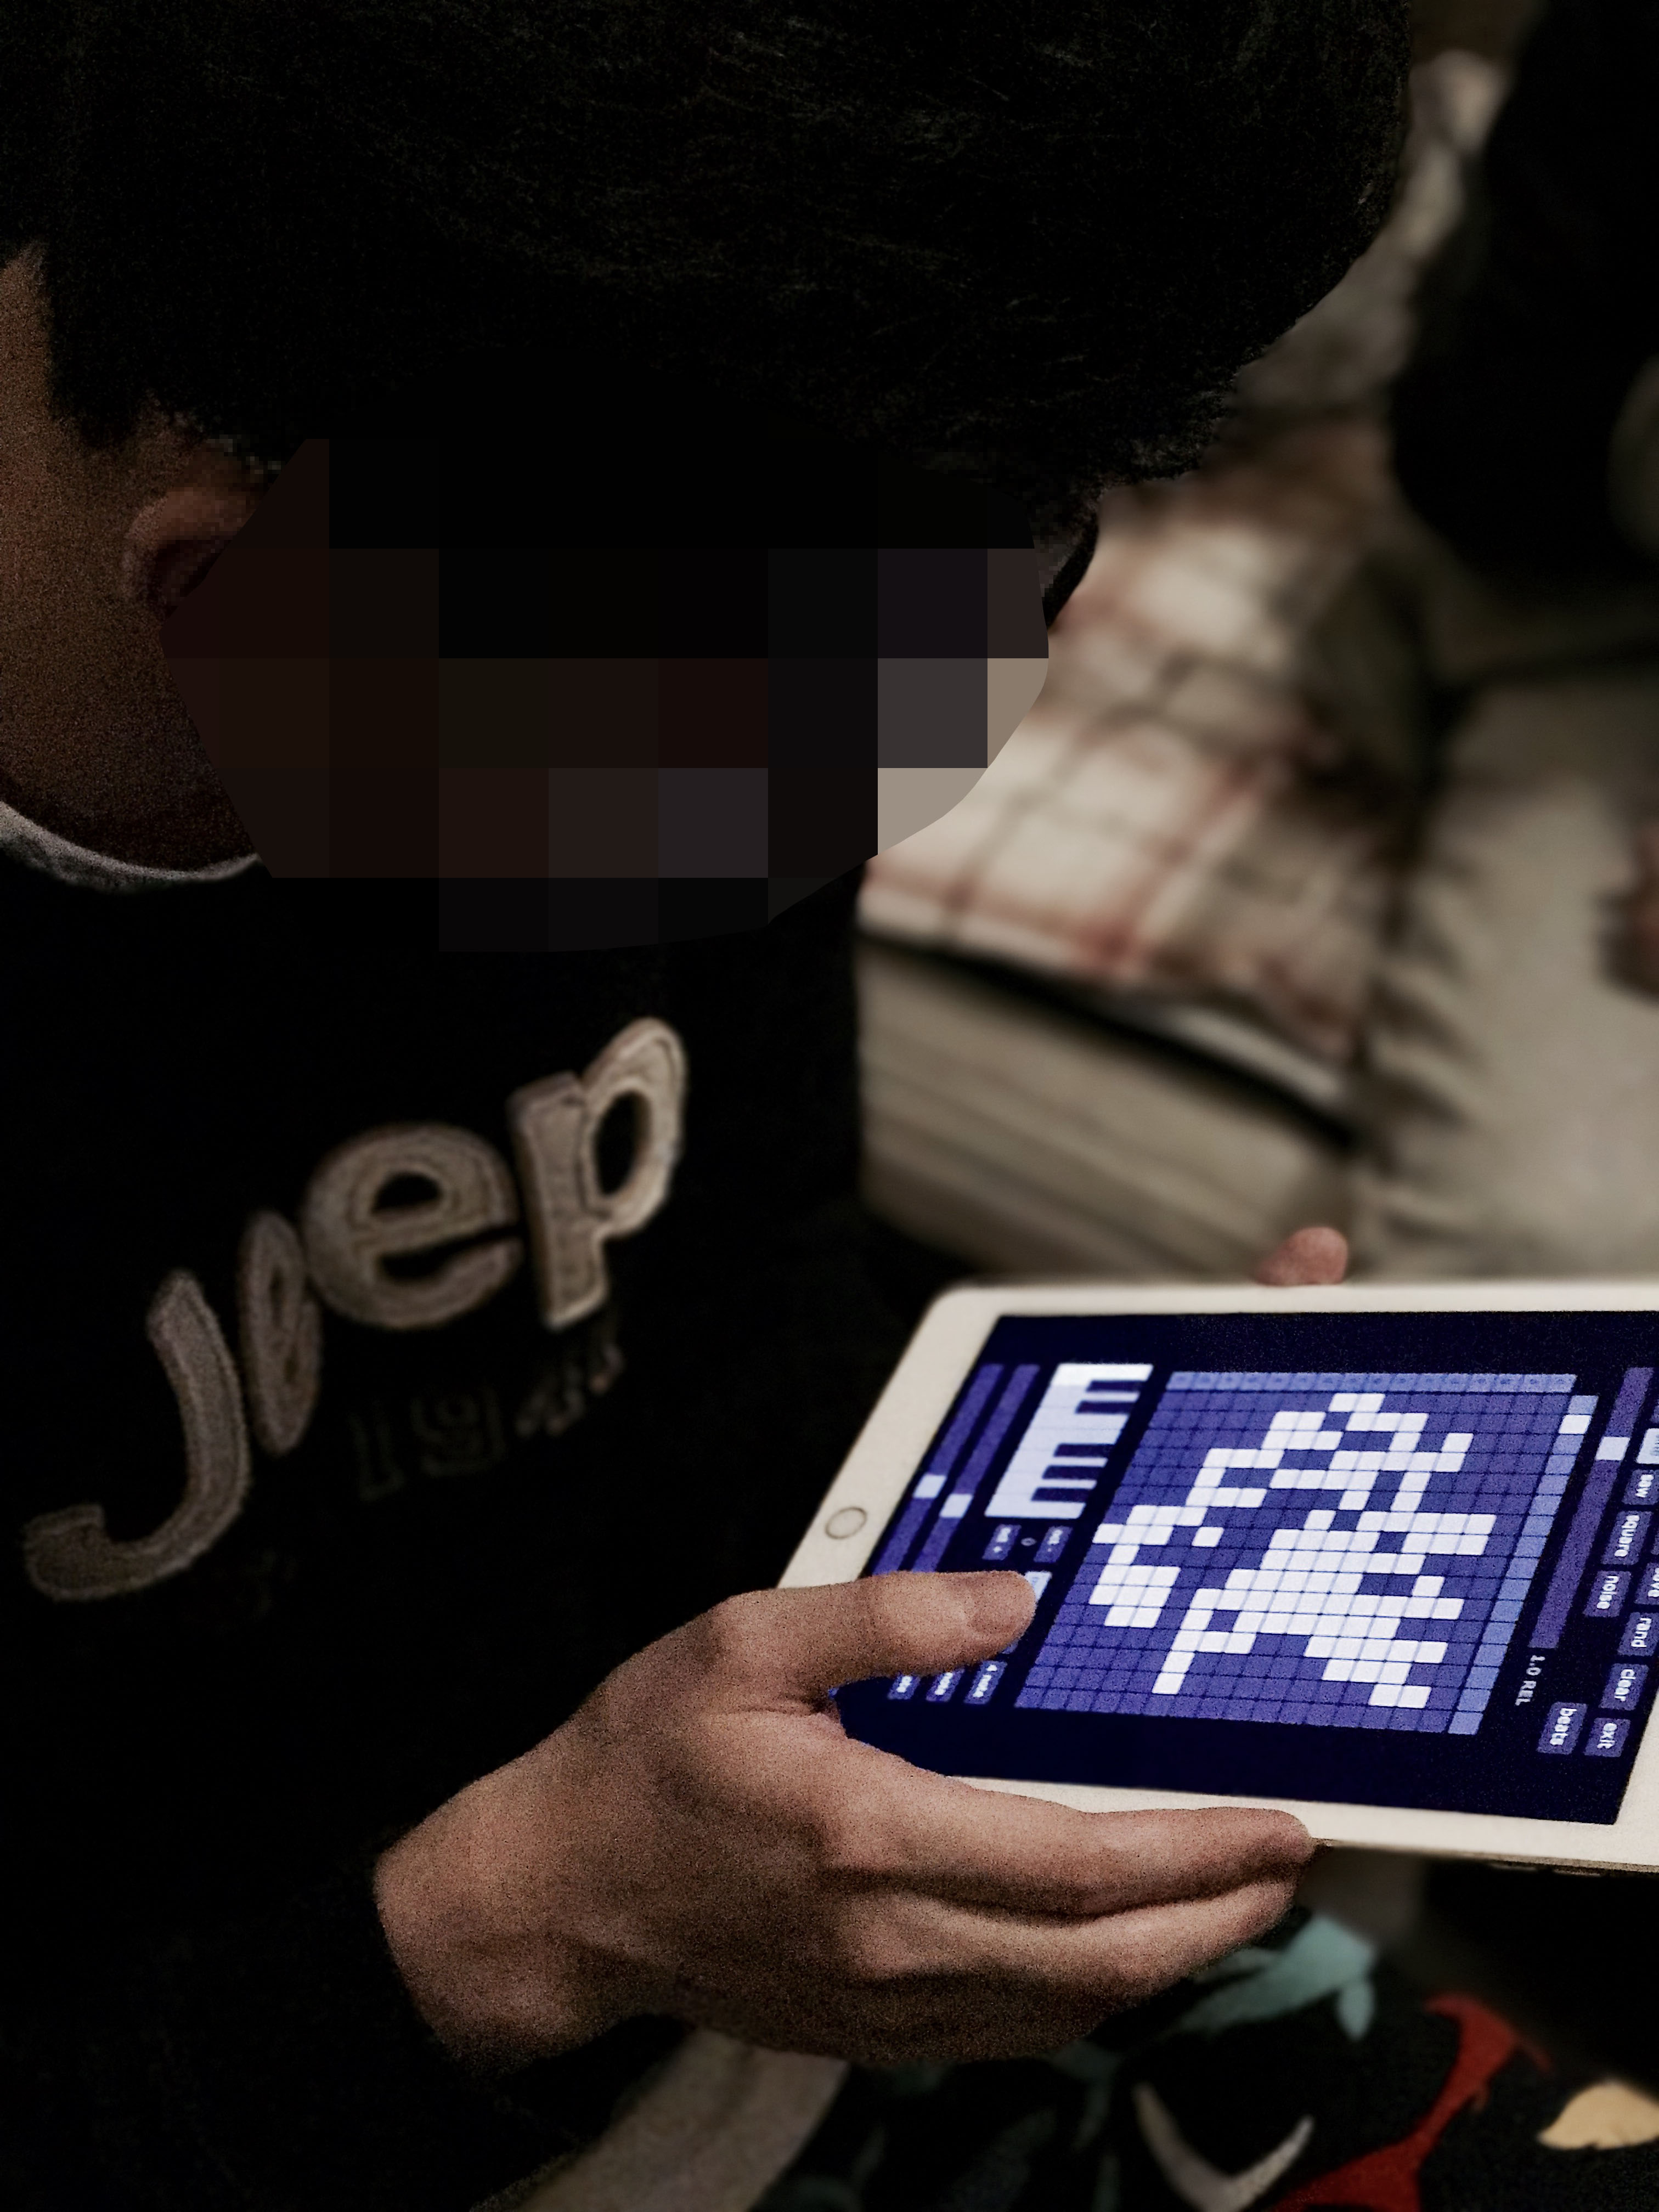
\includegraphics[width=6cm]{images/Participant}
  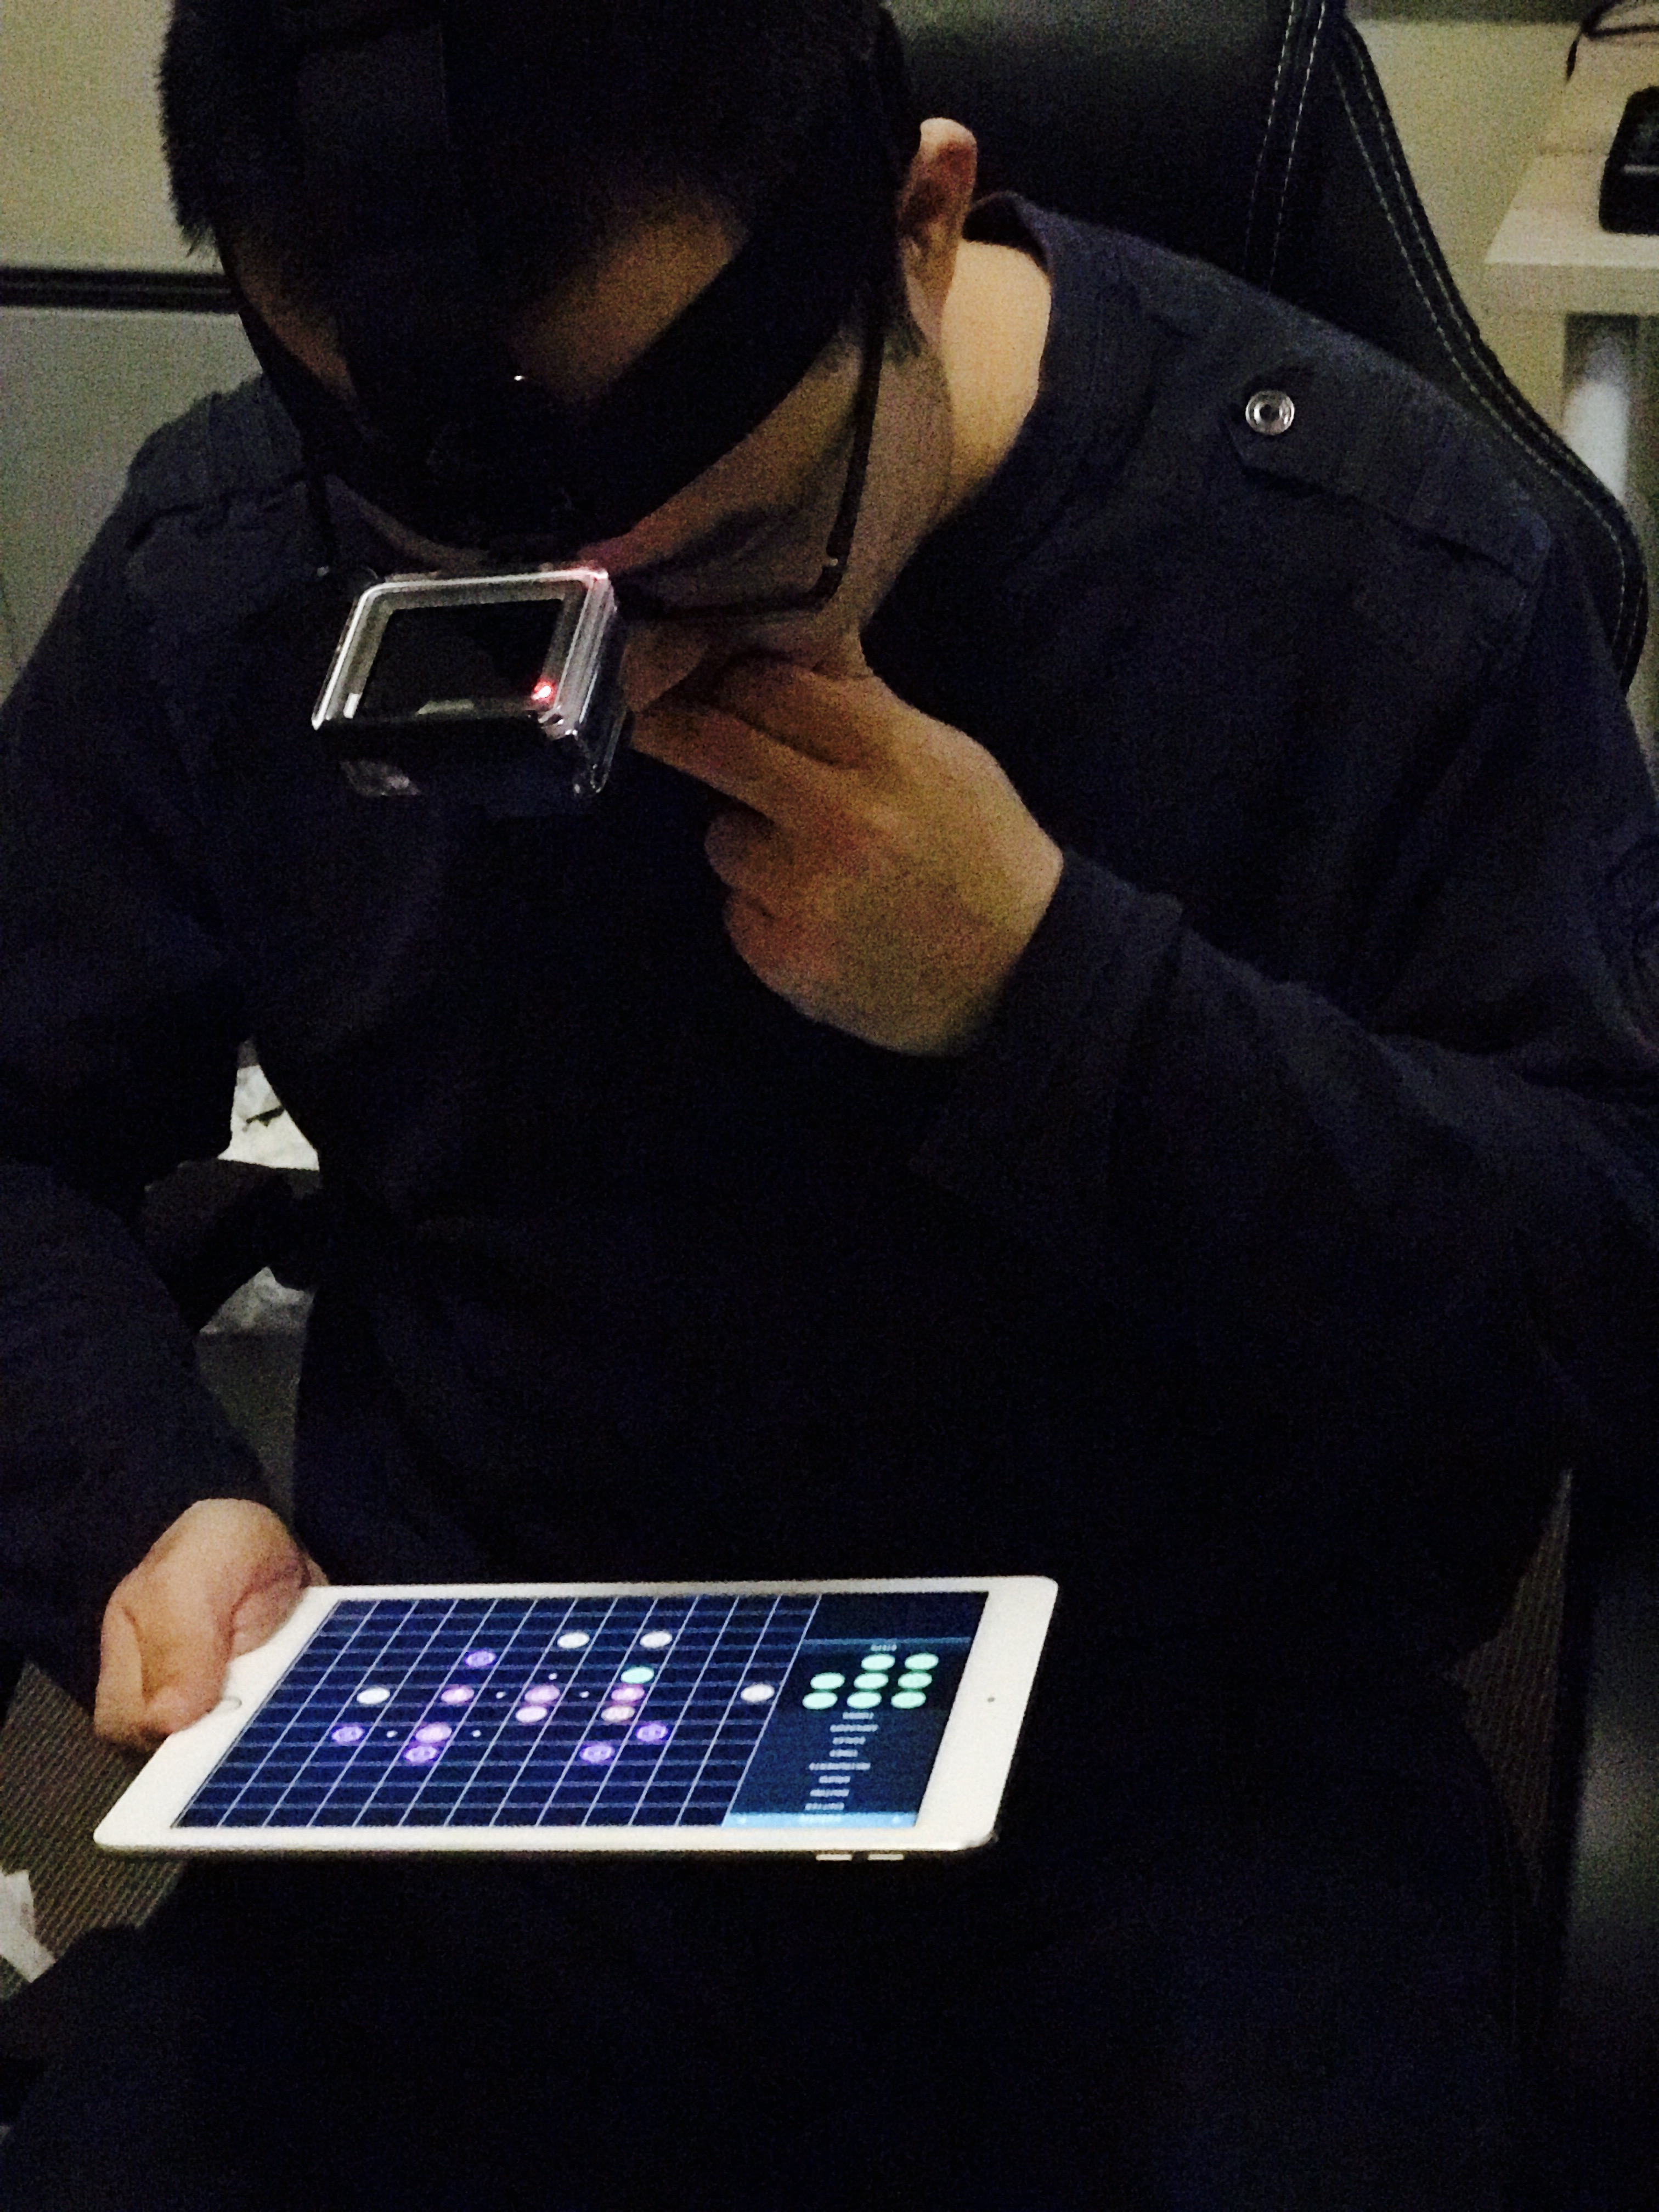
\includegraphics[width=6cm]{images/Participant2}
  \centering
  \caption{Participants test on the music sequencer on iPad}
  \label{fig: participant}
\end{figure}
\bigskip

\section{User Study Process}

The duration of the user study was planned as approximately one hour. The first fourty-five minutes was the try-on section which quantitively analyzed the interface (see \ref{subsec: play on}). In the last fifteen minutes, an interview was designed for qualitative analysis purpose (see \ref{subsec: interview}).

\subsection{Apps try-on}
\label{subsec: play on}
In this try-on section, all the participants were asked to play on the selected music sequencer applications on iPad. For each apps, musicians were given 15 minutes to explore the apps by themselves, and assistance was given only in request. The suggested time allocation was given as: in the first five minutes try to figure out the how it works, then impovise with the apps in the next ten minutes. After trying on each sequencer application, participants will be given a questionnaire with 10 questions to decide their feelings on the app in terms of expressivity, control and aesthetic(see Appendix \ref{app: Appendix B}).


\subsection{Interview}
\label{subsec: interview}
Participants were intervied at the end of the user study. The main purpose of the interview is to find out the reason behind their decision on the questionnaire. Besides, the music background of participants such as \textit{\textquotedblleft{how many years of music training}\textquotedblright} were recorded for further analysis. The sample question was given in the appendix \ref{app: AppendixC}.

In order to acquire the deeper reason, all the interview followed the same procedure: 1) Since the majority of the participants did not know music sequencer before, they were asked to describe the similarities among the three different music sequencer applications, and then defined what is music sequencer. which was designed to help them to form a general idea of music sequencer. 2) After that, interviewees were asked to choose their favourite application based on different scenario. Also, the interviewee needed to give reasons why certain music sequencer application was better than another. 3) In the final step, all the questions shifted to an abstract level, where they were asked whether music sequencer application on iPad were an instrument ,and what features that made them thought it is or it is not an instrument.The interviews were recorded on video and audio based on the participants agreement. The recording lasted between 10 to 20 minutes.

\section{Results}

\emph{My supervisor (Dr. Ben Swift) assisted in the preparation of the graphs
and statistical tests discussed in this section.}

\subsection{Quantitative Results}

In total, 600 satisfaction items from twenty participants were extracted from the questionnaire. The raw data was recorded on an Excel workbook (see Appendix \ref{app: Appendix D}). An overview of the participants response on the 10 questions with the selected music sequencer application is given in Figure \ref{fig: result_response}.

\begin{figure}[h]
 \centering
 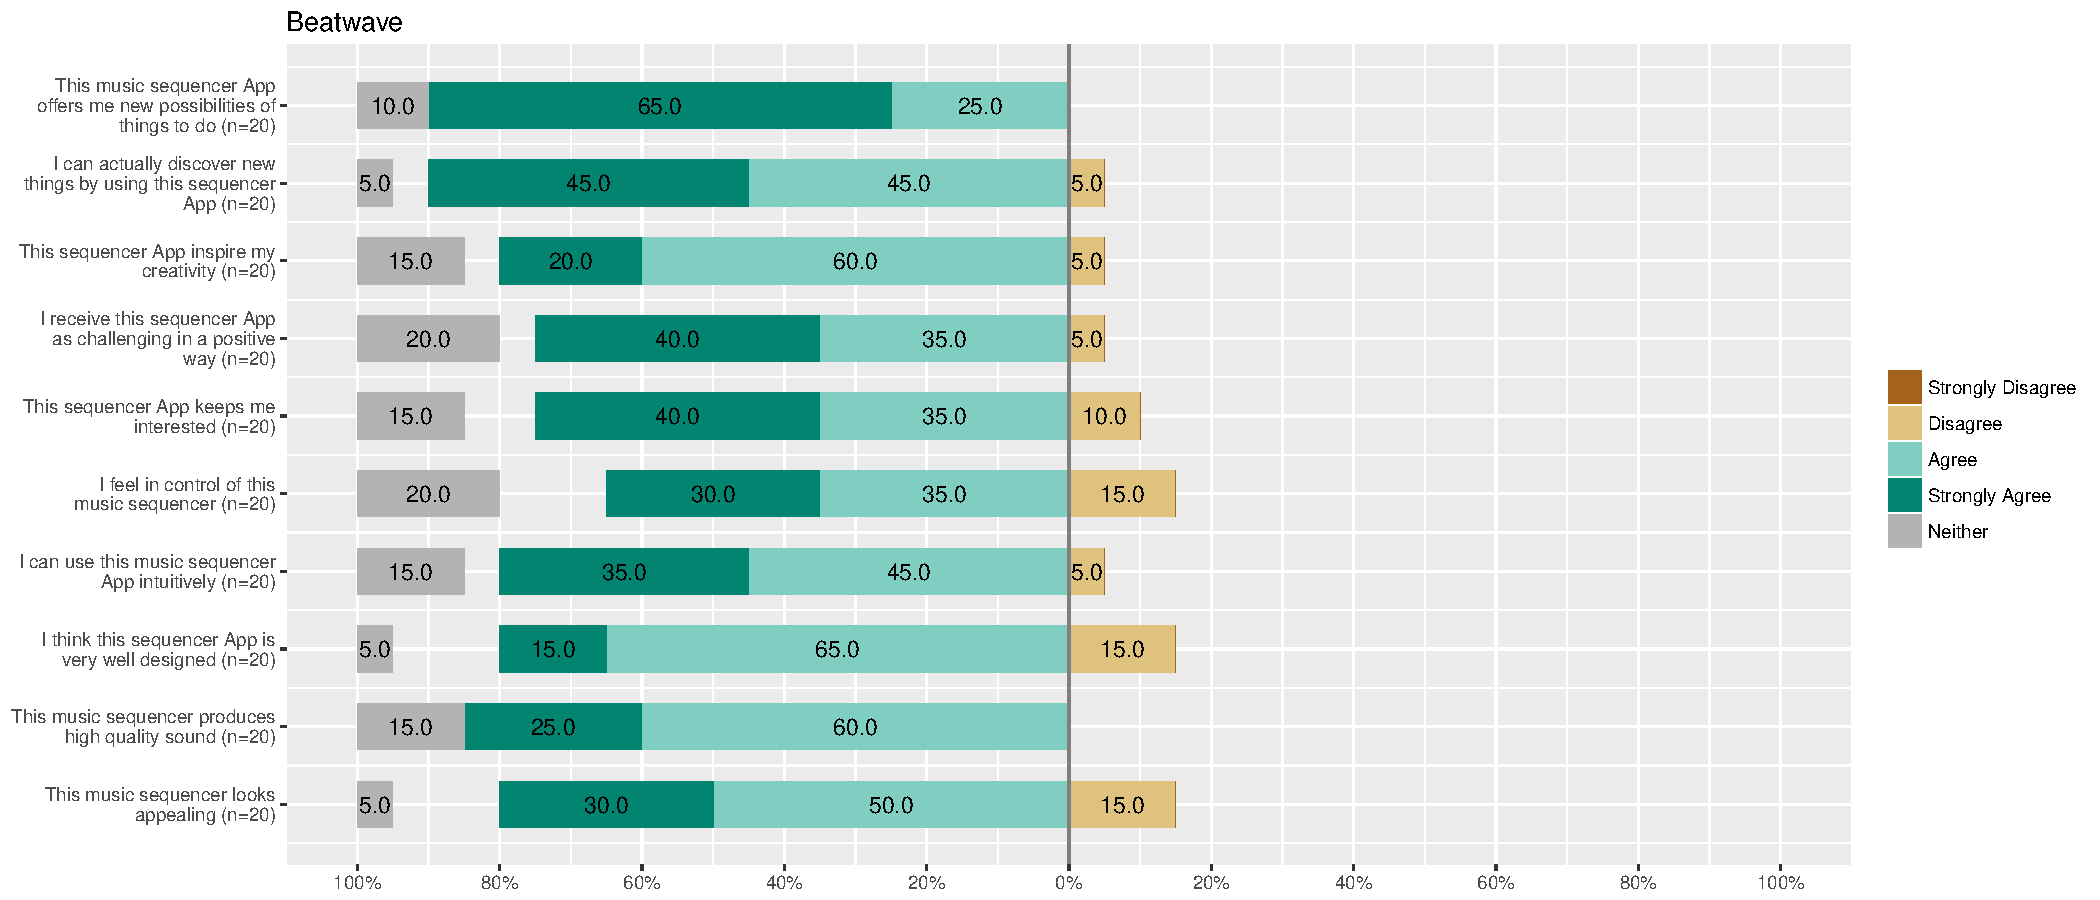
\includegraphics[width = \textwidth]{images/Beatwave.pdf}
 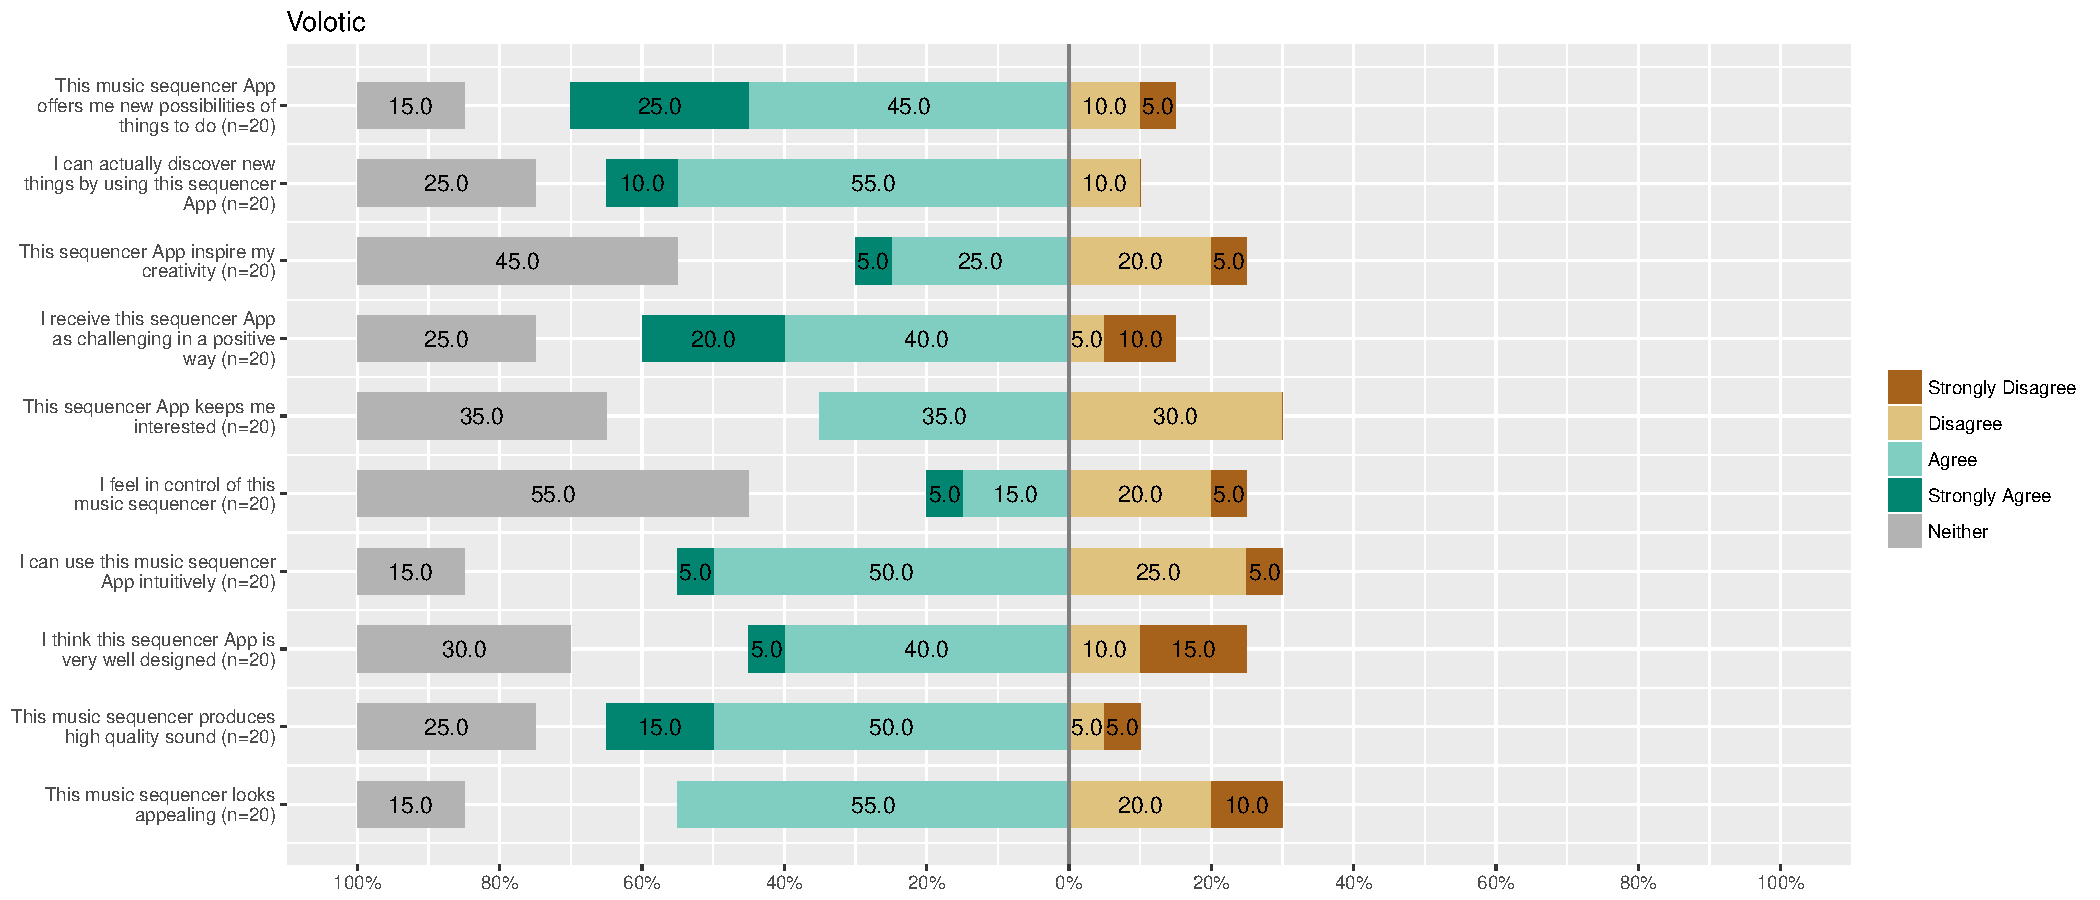
\includegraphics[width = \textwidth]{images/Volotic.pdf}
 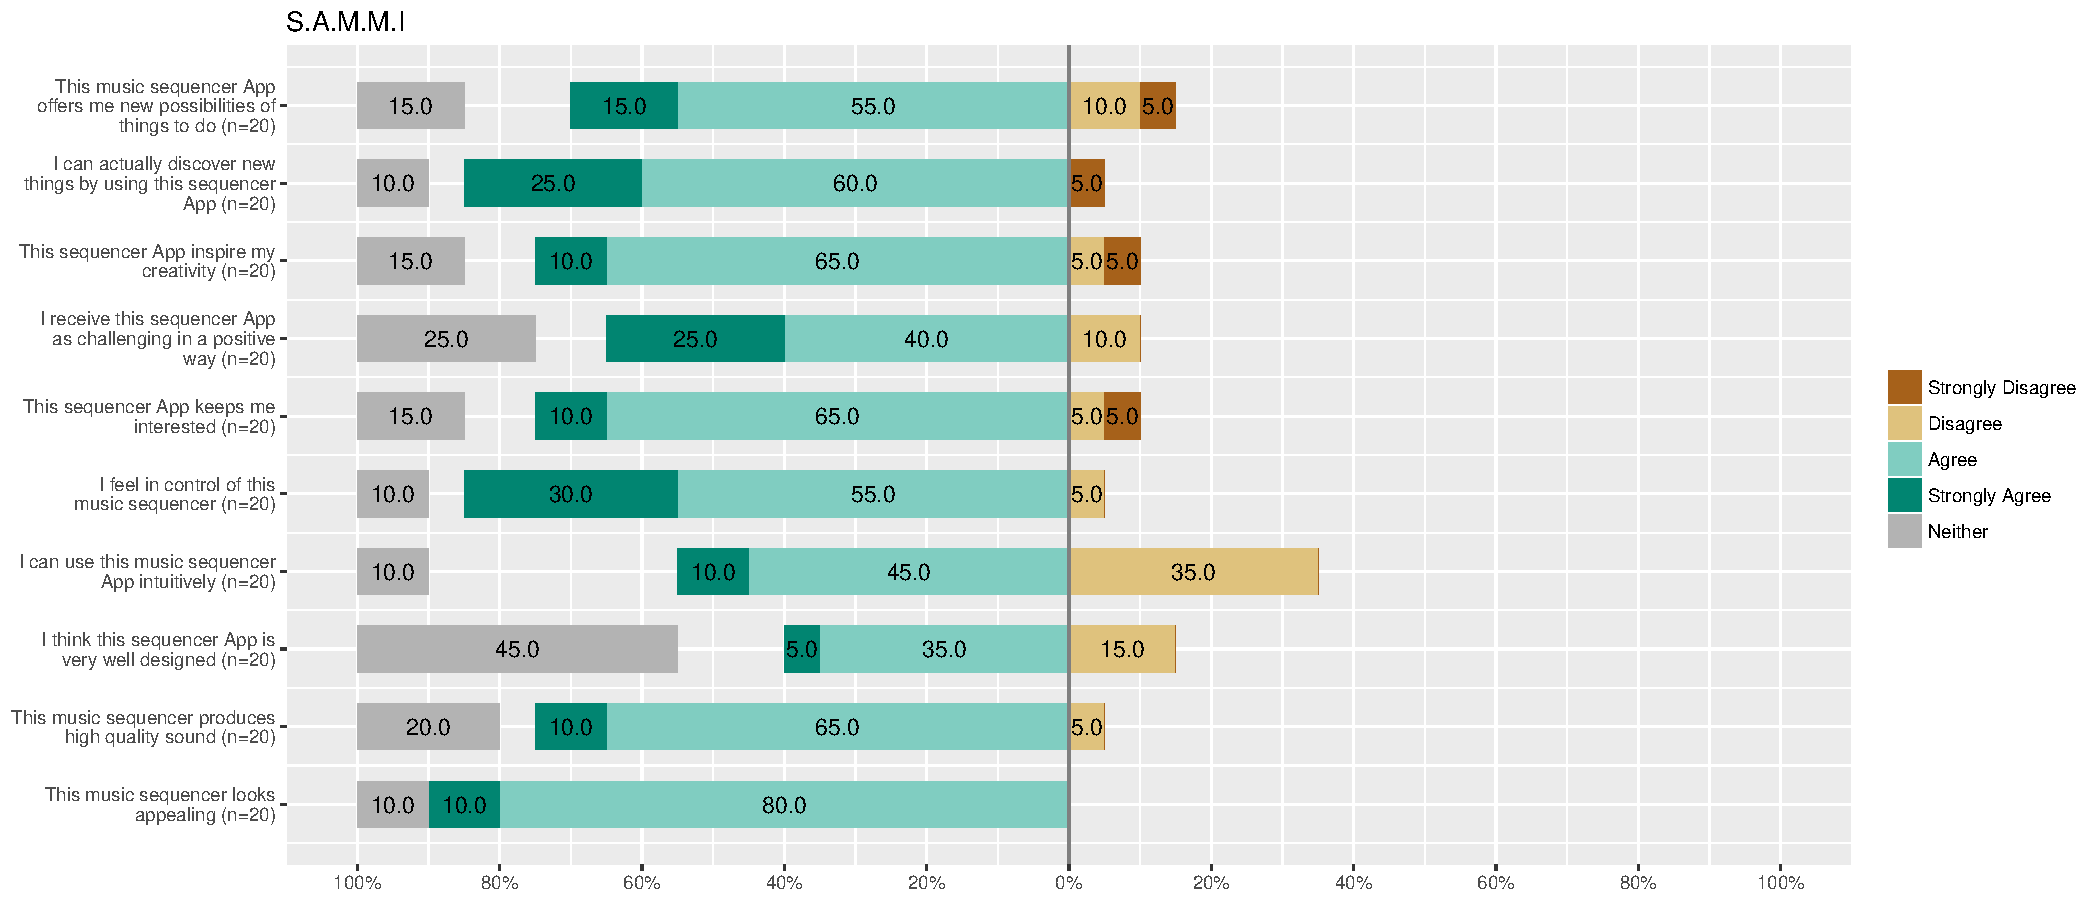
\includegraphics[width = \textwidth]{images/SAMMI.pdf}
 \caption{Participants response on Beatwave, Volotic and S.A.M.M.I}
 \label{fig: result_response}
\end{figure}

\subsection{Qualitative Results}

\begin{table}[h]
  \centering
  \begin{tabular}{ |p{2cm}|p{3.2cm}|p{3.2cm}|p{3.2cm}|}
   \multicolumn{4}{l}{} \\
   \hline
   Types & Expressivity  & Control  & Aethetic \\
   \hline
   Traditioanl & $\bullet$ can not fully express myself & $\bullet$ very easy to control & $\bullet$ the interface is dull\\
   & $\bullet$ don't have too much options &  $\bullet$ intuitive design & $\bullet$ not appealling\\
   & & &\\
   \hline
   Multi-track  & $\bullet$ inspire creativity & $\bullet$ not easy to get start & $\bullet$ the interface is awesome\\
   & $\bullet$ a lot of options& $\bullet$ the layout can be confusing & $\bullet$ the visual  is very helpful\\
   & & &\\
   \hline
   Novel & $\bullet$ inspire creativity in some degree & $\bullet$ very condusing & $\bullet$ it looks interesting\\
   & $\bullet$ it's fun & $\bullet$ would be better with with an instruction & $\bullet$ the interface looks like a game\\

   \hline
  \end{tabular}
  \caption[l]{ Musicians opinions summarised from the interview (grouped with the types of interface)}
  \label{tab: suduko}
\end{table}

\bigskip


% The result in this section is based on the information extracted from the interview. According to participants music-training background and the type of instruments they mainly used, we seperated the musicians into three groups: Group One (Playing traditional instruments but with less than three years formal music trainning), Group two (Playing traditional instruments but with more than three years formal music trainning), Group three (Playing electronic instruments and had more than three years formal music trainning). The reason why we don't have a group for musicians who play electronic instruments but less than three years formal music training is all the participants who play electronic instruments has many years experience in playing traditional instrument before.
%
% \textbf{Group \Romannum{1}.} Participants in this group have less experience in music in general, comparing with other two groups. They found \textit{S.A.M.M.I} was very easy to use becasue of the intuitive design of interface. Although \textit{S.A.M.M.I} didn't provide much options in terms of different sounds and adjustment on the sound effect, it was complex enough for them to discovery most of the possibilities. Besides, thanks to the annotation of different pitch, \textit{S.A.M.M.I} is the only application that they were able to create a short piece of melody, such as \textquotedblleft{Super Mario}\textquotedblright and \textquotedblleft{Mary Had a Little Lamb}\textquotedblright.
%
% The comments on \textit{Beatwave} were mainly focused on the layout of different tracks. They agreed combining severl layers of music together was definitely an improvement, but this design pattern made it more difficult to control comparing to the single-track interface design of \textit{S.A.M.M.I}. Furthermore, participants in Group One believed the visual effect of \textit{Beatwave} gave them a positive feedback. The rippling effect of the current note helped them tracked down the progress of the music.
%
% \textit{Volotic} was recognized as the most difficult application to create music. Most participants in this group thought \textquotedblleft{It's more like a game rather than an instrument}\textquotedblright. But they still thought it was a very good practice and could potentially used to help kids generate interest in music.
%
% \textbf{Group \Romannum{2}.} Participants in this group were musicians have more than 3 years professional trainning in traditional instruments like piano. In general, they have relatively deeper understanding of music. Although,\textit{S.A.M.M.I} got most credit by providing explict display of pitch, most musicians in this group didn't rely on it. Because they could accurately justify the pitch by hearing the sound. Besides, the intuitive design of \textit{S.A.M.M.I}'s interface was considered to be redundant. They thought the interface could be further simplified. However, one musician bought up an interesting comment on \textit{S.A.M.M.I}. He fully untilised the explicit layout of control panel by chaning the flavour of music continuously, and explored the possibility of live performing with \textit{S.A.M.M.I}
%
% \textit{Beatwave} was recognized as an upgrade version of \textit{S.A.M.M.I} by adding new features such as multi-track and visual feedback. Even though \textit{Beatwave} took musicians in Group Two longer time to learn, it provided them a larger platform to express themselves. Because musicians in this group mainly focused on traditional instruments, they tend to duplicate the melody they learned before. Thus, an electronic version of \textquotedblleft{Song of Joy}\textquotedblright was created. And during this process, they found the interface of \textit{Beatwave} was designed to focus on a larger picture of music as a whole rather than create a short piece of melody. Another interesting finding was interviewee in this group didn't give much credit on the visual feedback, but considered it as decoration which made the user interface(UI) looked fancy.
%
% Same with the participants in Group One, musicians in this group thought \textit{Volotic} was \textquotedblleft{very confusing}\textquotedblright. In spite of several demos provided in the beginning, almost all the musicians still found it hard to figure out how \textit{Volotic} worked. Furthermore, timing in \textit{Volotic} was controled by the time that signal(little dots) traveled from one unit to another. However, it turned to be diffcult to control when there were several little dots travelling on the screen.
%
% \textbf{Group \Romannum{3}.} Unlikes the previous groups, musicians in this group had exposed to electronic music for a long time, and they all had experience in using a music sequencer hardware or something similar before. Thus, people in this group had certain knowledge on music sequencing, and had experience on making electronic music. The experience on electronic music let those musicians provided suggestions from a more professional perspective. For them, \textit{S.A.M.M.I} was like an instrument for beginner and witch cannot let them fully express themselves.
%
% Most of the conversation was around \textit{Bearwave}. The implementation of multi-track assisted musicians to compose music by editing differet layers. What's more, with the management system to handle different sections of music, it helped musicians to extend the length of their works. Also, considering the appearence of the electronic instruments are becoming more colorful and shiny, the visual effect of \textit{Beatwave} made the interface more appealing compaing to the other two applications. However, there were demand on integrating synthesizer into \textit{Beatwave} so as to have more freedom on sound mixing. An alternative way proposed by one of the musicians was developed an input/output system, which potentially made the application more practical.
%
% The opinions on \textit{Volotic} in group three were more open companing with the other groups. Musicians in this group were tend to give credite for the innovative design of \textit{Volotic}'s interface. Despite the fact that the name of symbols were unclear, they still believed they could make some interesting music with \textit{Volotic} if more time been given.

\subsection{Discussion}

When dealing with statistical significance and Likert scale responses,it is important not to make assumptions of the data which are not true in the likert case\citep{norman_likert_2010}. The Aligned Rank
Transform\citep{wobbrock_aligned_2011} (ART) has become popular in the CHI community to perform non-parametric factorial analyses of likert responses. Although finding statistical significance is not the main
point of this user study, an ART was performed (using the R ARTool package\citep{matthew_kay_2016_48543}) to see if there was any difference in the responses between the apps. Table \ref{tab: p-value} shows the results after applying a Bonferroni correction to account for multiple tests. In the table the questions in shade were regarded as not significant, because the adjusted p-value of these two question were greater than 0.05.

\bigskip
\begin{table}[ht]
\rowcolors{2}{gray!25}{gray!25}
\begin{tabular}{p{12cm} p{1.5cm}}
 \hline
 \rowcolor{gray!50}
Questions & adjusted \textit{p-value} \\
\hline
\hiderowcolors The instrument allows me to be creative & 0.0014 \\
\hiderowcolors The instrument responds well to my actions & 0.0234 \\
\hiderowcolors I can rely on the instrument when playing it & 0.0009 \\
\showrowcolors I have fun playing the instrument & 0.3093 \\
\hiderowcolors The instrument allows me to express myself & 0.0010 \\
\hiderowcolors I can control the sound appropriately & 0.0009 \\
The instrument pleases me sound-wise & 0.0121 \\
\hiderowcolors I feel the urge to play the instrument again & 0.0486 \\
\showrowcolors The instrument allows me to be engaged when I'm playing it & 0.1523 \\
\hiderowcolors I can recognize that the instrument responds well to my playing & 0.0006 \\
\hiderowcolors
\hline
\end{tabular}
\caption{Questions with adjusted p-value.}
\label{tab: p-value}
\end{table}

From the statistic results extracted from the questionnaire, it is clear to say that the multi-track interface represented by \textit{Beatwave} is the most popular design among musicians. By contrast, the non-traditional interface represented by \textit{Volotic} received most of the nagative comments.

Considering the factor each question belong to (see Table \ref{tab: questionnaire}), we can look in details of what specific aspect an interface good at. In Figure \ref{fig: EFP}, statistic result for questions belong to \textit{EFP} were grouped together. Apparently, \textit{Beatwave} was the best applcation to encourage musicians creativity. And \textit{Volotic} was slightly better than \textit{S.A.M.M.I} in this category. In enjoyment category, \textit{Beatwave} still gathered most of \textquotedblleft{Strong Agreement}\textquotedblright. But \textit{Volotic} was not that fun compaied with \textit{S.A.M.M.I}. For the expressiveness of the applications, \textit{Beatwave} and \textit{S.A.M.M.I} were quite similar, the only difference was musicians had stronger feeling on \textit{Beatwave}. However, opinions on \textit{Volotic} were equally distributed, it looked like musicians had a substential differences on whether the interface of \textit{Volotic} supported them to expressed themselves.
%
% \bigskip
% \begin{figure}
% \begin{minipage}[b]{0.5\textwidth}
% 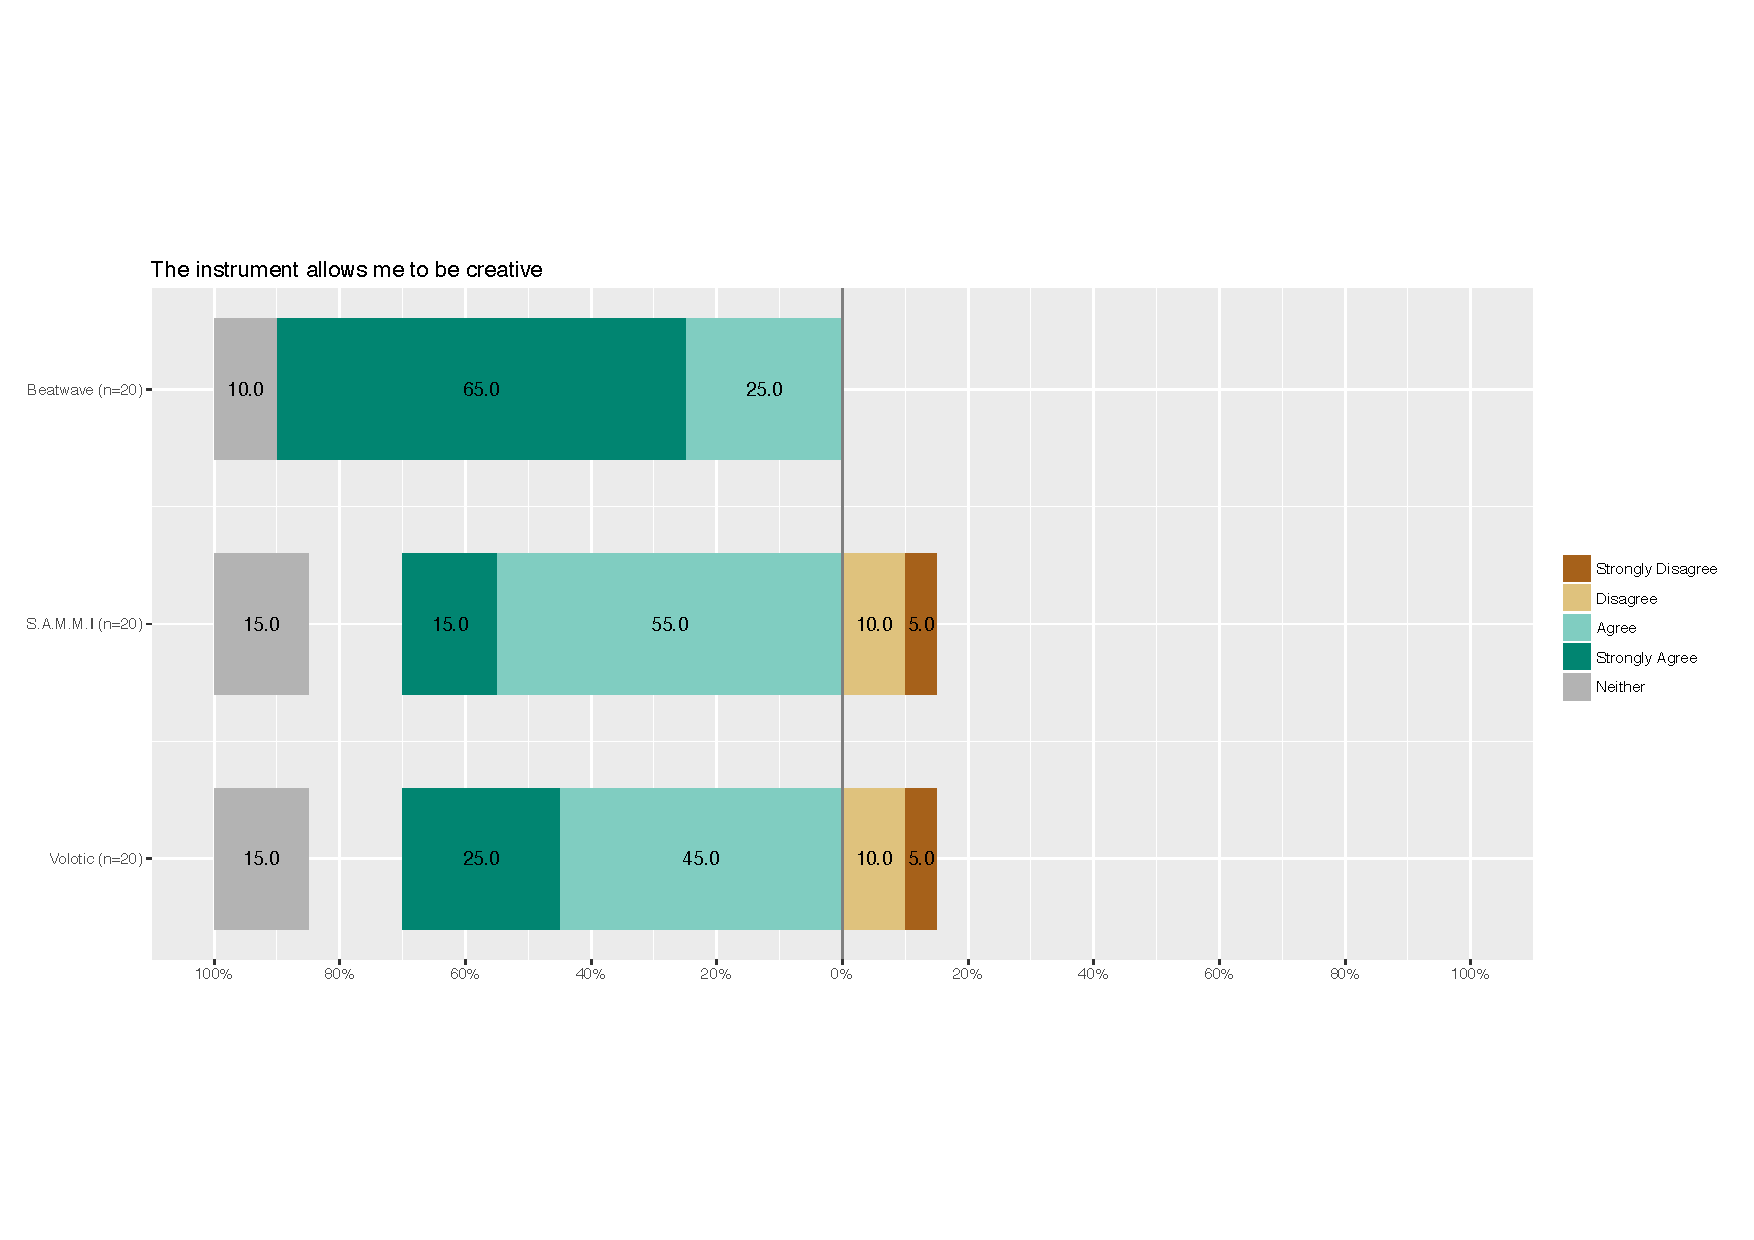
\includegraphics[width=\linewidth]{figs/Q1.pdf}
% \end{minipage}
% \begin{minipage}[b]{0.5\textwidth}
% 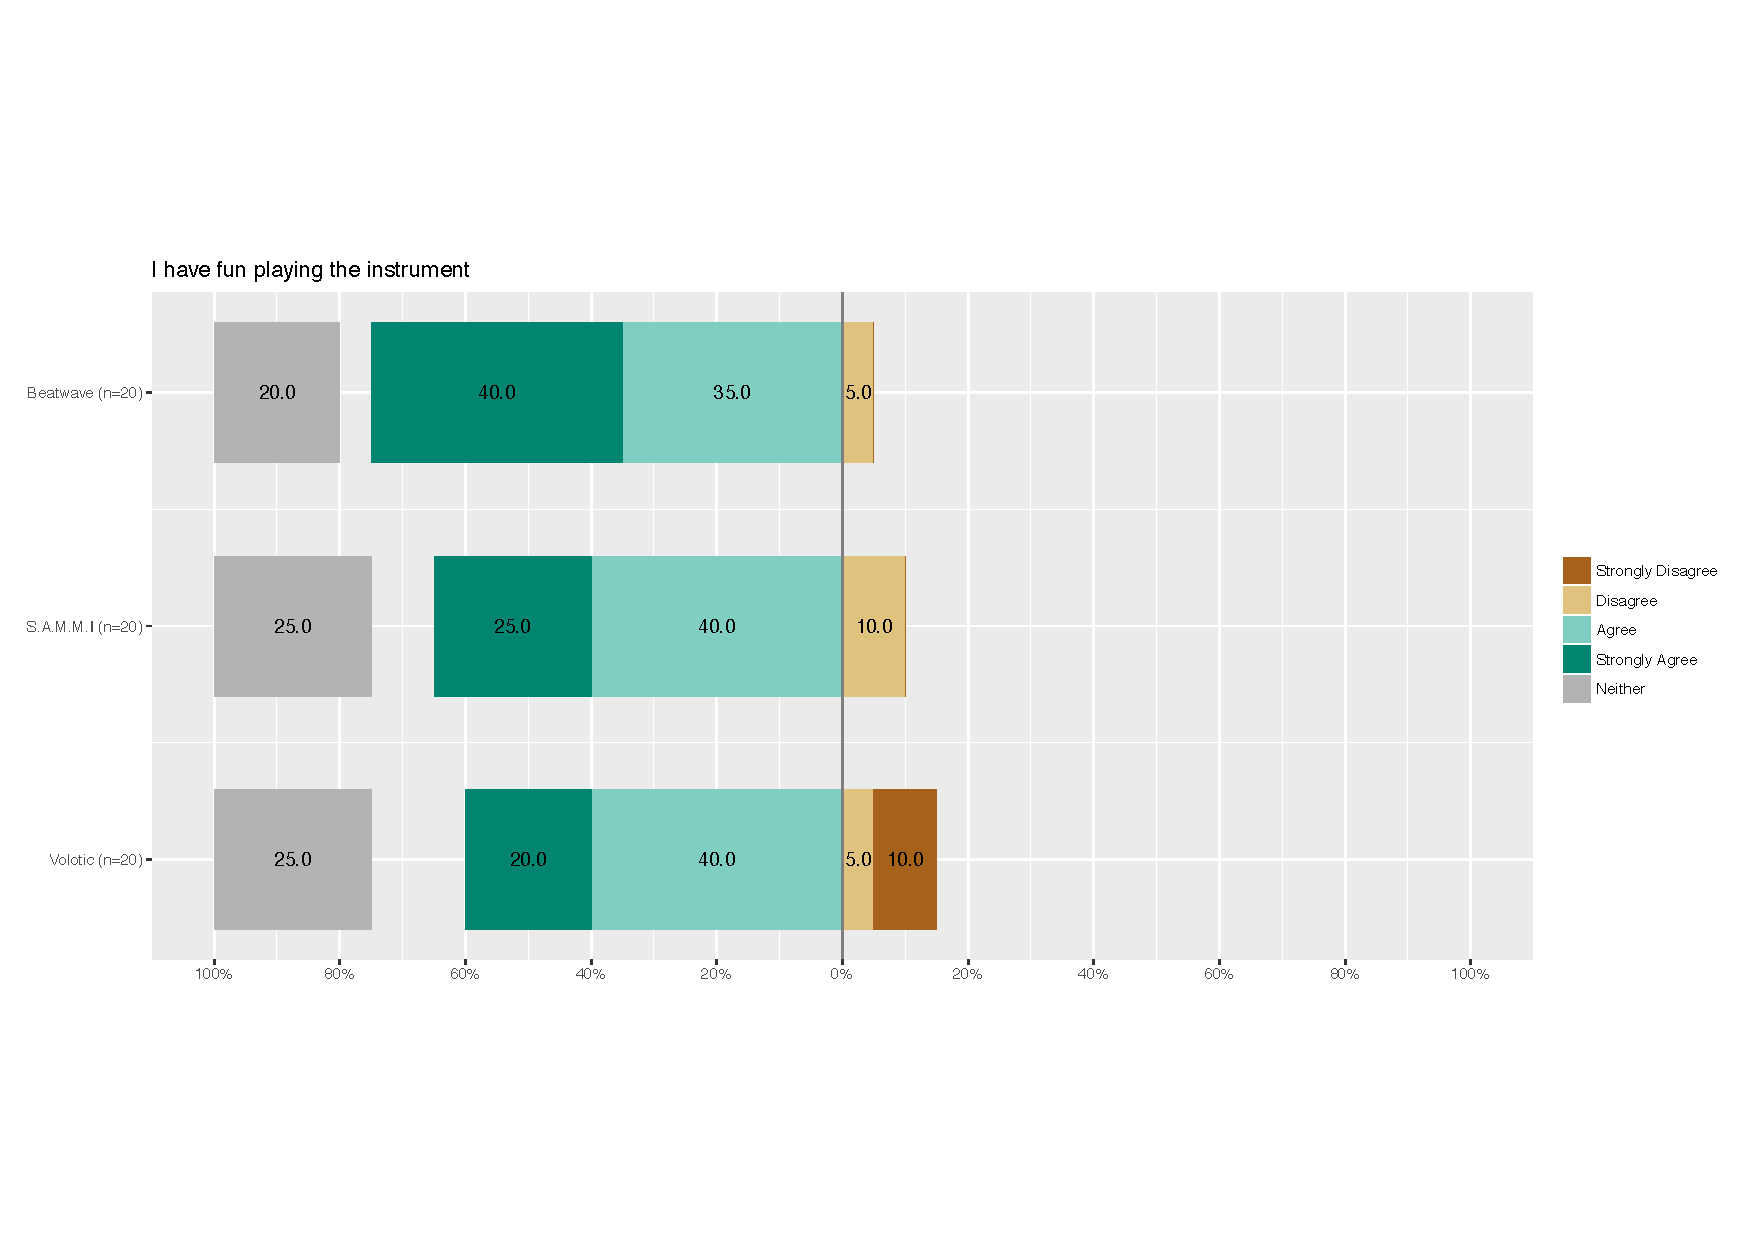
\includegraphics[width=\linewidth]{figs/Q4.pdf}
% \end{minipage}
%
% % \hspace{\fill}
%
% \begin{minipage}[b]{0.5\textwidth}
% 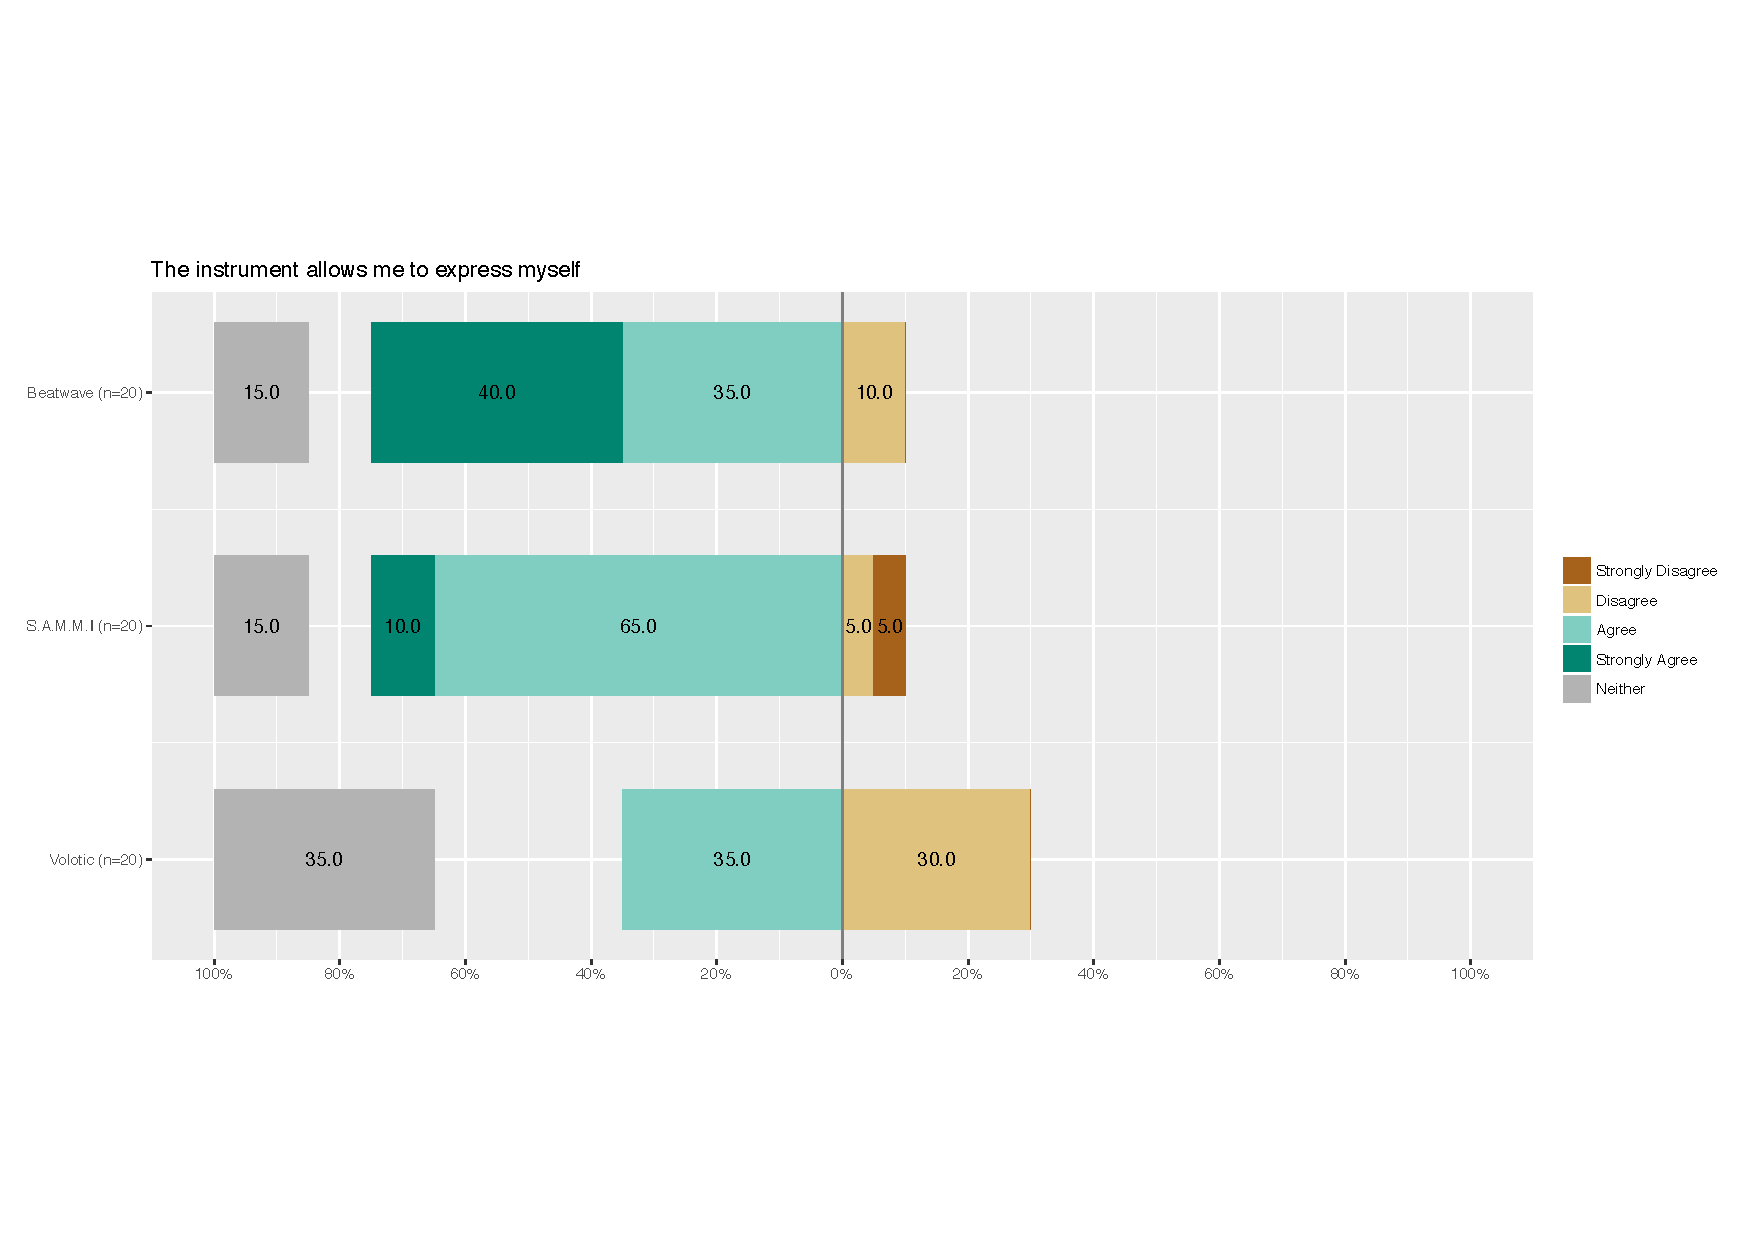
\includegraphics[width=\linewidth]{figs/Q5.pdf}
% \end{minipage}
% \begin{minipage}[b]{0.5\textwidth}
% 
\includegraphics[width=\linewidth]{figs/Q0.pdf}
% \end{minipage}
%
% \caption{Statistic results for questions belong to \textit{EFP}}
% \label{fig: EFP}
% \end{figure}
% \bigskip


\clearpage
